%%%%%%%%%%%%%%%%%%%%%%%%%%%%%%%%%%%%%%%%%
%%% Guidelines
%%%%%%%%%%%%%%%%%%%%%%%%%%%%%%%%%%%%%%%%%

\clearpage
\section{Guidelines}
\label{sec:guidelines}

%%%%%%%%%%%%%%%%%%%%%%%%%%%%%%%%%%%%%%%%%
%%% Section content, please change!
%%%%%%%%%%%%%%%%%%%%%%%%%%%%%%%%%%%%%%%%%
\subsection{Process Overview}
\label{sec:latex-style-files}

\newcommand{\macro}[1]{{\tt \textbackslash #1}}

Use the following macros to provide the required information in the deliverable (located in the \texttt{deliverable.tex} file):


\begin{itemize}
    \item \macro{ProjectAcronym\{\}}, \macro{ProjectFullTitle\{\}}, \macro{ProjectRefNo\{\}}: these are pre-set to the obvious values
    \item \macro{delivWP\{\}}: the deliverable WP
    \item \macro{delivWPName\{\}}: the deliverable WP name, as appears in the DoA
    \item \macro{delivNumber\{\}}: the deliverable number, Dx.y
    \item \macro{delivName\{\}}: deliverable's title, as appears in the DoA
    \item \macro{delivShortTile\{\}}: short title of the deliverable
    \item \macro{delivResponsible\{\}}: responsible partner (participant short name)
    \item \macro{delivVersion\{\}}: version as vn.n
    \item \macro{ContractualDate\{\}}: due date
    \item \macro{ActualDate\{\}}: date of submission
    \item \macro{delivDissLevel\{\}}: PU or SEN
    \item \macro{delivType\{\}}: Report, Data Management Plan, Demonstrator, Other (choose one)
    \item \macro{delivAuthor\{\}}: Name(s) of the Deliverable Leader(s) (also participant short name(s)
    \item \macro{delivFPAuthor\{\}}: Names of co-authors (also participants short names)
    \item \macro{delivReviewers\{\}}: Names of reviewers (also participants short names)
    \item \macro{delivStatus\{\}}: (d)raft, (f)inal, or (s)ubmitted
    \item \macro{delivKeywords\{\}}: List of free keywords relevant to the deliverable
    \item \macro{istChange\{\}\{\}\{\}\{\}}: for setting deliverable revisions items. The first argument is the date, the second is the deliverable's version number, the third, the author's name, and the fourth the summary of changes made. You may add as many of these commands as you like. They will be stored and added to the table on   the second page.  
\end{itemize}

The steps are the following: 

\begin{enumerate}
    \item \textbf{Deliverable Setup} -  The deliverable setup starts from the \texttt{deliverable.tex} file. In this file, you have to set the above macros to provide the required information in the deliverable.
    \item \textbf{Sections of the Deliverable} - Inside the \texttt{sections} folder, there are the various sections of the deliverable. Start from the introduction (\texttt{introduction.tex}), then move on to the executive summary (\texttt{summmary.tex}) and the abbreviations (\texttt{abbreviations.tex}). After that, proceed to write the main text for the deliverable using the \texttt{mainbodyofthedeliverable.tex} file. 
    \item \textbf{Conclusion and Appendices} -  For the conclusions, use the \texttt{conclusion.tex} file. For the appendices (if any) use the \texttt{appendix-a.tex} and \texttt{appendix-b.tex} files.
    \item \textbf{\textit{Note:}} If you want to exclude a section (for example, the appendices), all you have to do is comment out the ``corresponding loader'' in the \texttt{deliverables.tex} file. Example: Comment the\texttt{\textbackslash input\{sections/appendix-a\}} from the \texttt{deliverables.tex} file, and Appendix-A will disappear from the PDF.
\end{enumerate}


\subsection{Abbreviations}
\label{sec:report-titles}


To include abbreviations in the document, first declare them in \texttt{sections/abbreviations.tex}. To make them appear in the list, use the \texttt{\textbackslash ac\{\}} command.

\textbf{Example:} \ac{EC}


\subsection{File Naming}
\label{sec:file-naming}

The project will generate many documents (deliverable reports) and versions of these deliverables. It is beneficial to consistently use an agreed file naming format. 

\textit{CoEvolution-Dnn-ShortTitle-Status-vn.n.Extension}

Please note that file naming will be handled \textbf{automatically} by providing the necessary macros, as discussed in Section \ref{sec:latex-style-files}.

\begin{itemize}
	\item Notice the hyphen between the various elements of the file name.
    \item {\bf \hyperride{}}: Each \hyperride{} deliverable should be preceded by the project acronym. Notice, there is only one correct spelling of the acronym: ‘\hyperride{}’. 
    \item {\bf Dn.n}: Indicates the deliverable identifier, e.g., ‘D34’ for ‘D3.4’ following the numbering of the \ac{DoA}. Notice, there is no dot between the two parts of the deliverable number.
    \item {\bf ShortTitle}: This should be based on the formal short title of deliverables but ‘contracted’ into a single (no spaces) character string using Java class naming convention, e.g., ‘ExploitationPlan’,  or ‘ProjectWebSite’. Avoid underscore, space and other unusual characters.
	\item {\bf Status}: 
	\begin{itemize}
		\item \textit{draft} = Draft Version – indicates that the drafting of the report is in progress; 
		\item \textit{final} = Final Version as checked and updated by the reviewers/WP leader/SPM/ PC; 
		\item \textit{submitted} = submitted version as submitted to the EC by the PC.
	\end{itemize}
	\item {\bf vn.n}: The version of the deliverable. The last version will be v1.0.
    \item {\bf Extension}: File extension, e.g., ‘pdf’ for Portable Document Format. 
\end{itemize}

Examples:

\begin{itemize}
    \item CoEvolution-D82-InternalCommunication-draft-v1.0.pdf
    \item CoEvolution-D84-QualityAssurancePlan-submitted.pdf
\end{itemize}



\subsection{Deliverable Revisions}
\label{sec:change-log}

The ``Deliverable Revisions'' table (page 2) is there to keep track of the changes made to the document. Whenever changes are made to the document, a new version should be created and the changes should be briefly summarised in the Deliverable Revisions. We anticipate a minimum of three phases of Deliverable Revisions entries. (1) The Deliverable Leader enters the changes as he/she develops the document. (2) The two reviewers register the changes made in the quality assurance phase. Once the Deliverable Leader passes the report on to the Project Coordinator, the status should be changed from ‘draft’ to ‘final’. (3) The Project Coordinator submits the report to the EC, the status should be changed from ‘final’ to ‘submitted’.

\subsection{Document Formatting}
\label{sec:document-formatting}

\subsubsection{Document sectioning}
\label{sec:headings}


There are 5 levels of depth for defining sections:

\begin{itemize}
    \item \texttt{\textbackslash section\{\}}
    \item \texttt{\textbackslash subsection\{\}}
    \item \texttt{\textbackslash subsubsection\{\}}
    \item \texttt{\textbackslash paragraph\{\}}
    \item \texttt{\textbackslash subparagraph\{\}}
\end{itemize}

Under each section, add a unique label for cross-referencing. 


\subsubsection{Tables}
\label{sec:tables}

An example table using the \LaTeX\ table feature is shown below (\Cref{tab:latextable}).

\begin{table}[htb]
	\centering
	\caption{Summary of properties of different modelling formalisms. The table below is produced using \LaTeX's {\tt table} environment.}
	\label{tab:latextable}
     \def\arraystretch{1.25}
	\begin{tabular}{|c|c|c|c|c|c|}
		\hline
		\rowcolor{gray!30} % Adds a light gray background to the header row
		& Static & Discrete & Deterministic & Qualitative & Coarse \\ 
	    \hline
	    DG & s &  & d & ql & c \\ \hline
	    BYN & s & d,c & s & qn & c\\ \hline
	    BNN & d & d & d & ql & c\\ \hline
	    GLN & d & c & d & qn & a,f\\ \hline
	\end{tabular}
\end{table}

The caption, as well as the table, should be centered using the \texttt{\textbackslash centering\{\}} command.

To add a caption to the table, use the \texttt{\textbackslash caption\{\}} command. 

Ensure that cross-references to tables are correct before submitting the deliverable. 

To cross-reference a table, first create the table using the LaTeX table feature, then use the \texttt{\textbackslash Cref\{\}} command to reference it.

In order to cross-reference a table, you must first add a \texttt{label} to the table. To add a label, use the \texttt{\textbackslash label\{\}} command (see the example table above).


Below is another table illustrated as an example, which uses specific column width dimensions. The table is structured with the following column widths: 6.5 cm for the second column, 3.8 cm for the third column, and 2.2 cm for the fourth column. This format can be used as a reference for structuring similar tables.

\begin{table}[htb]
	\centering
	\caption{CoEvolution Work Package Leaders}
	\label{tab:work_package_leaders}
      \def\arraystretch{1.25}	
       \begin{tabular}{|l|>{\raggedright}p{6.5cm}|p{3.8cm}|p{2.2cm}|}
		\hline
		\rowcolor{gray!30} % Adds a light gray background to the header row
		No & Name & Leader & Organisation \\
	    \hline
    	     WP1 & Project Management & Konstantinos Tserpes & ICCS  \\ \hline
    	     WP2 & Dissemination, Exploitation, Sustainability  & Andreas Miaoudakis  & CBRL \\ \hline
    	     WP3 & Specification / Requirements and CoEvolution
Architecture & Apostolos Fournaris  & ISI \\ \hline
    	     WP4 & AI model STR Assessment, Enhancement and
Context Awareness technology enablers & Ioannis Arapakis & TID \\ \hline
              WP5 & CoEvolution AI model lifecycle STR Security
Assurance and Monitoring & Sotiris Ioannidis & DIE  \\ \hline
    	     WP6 & Integration, evaluation and project outcomes & Aris Lalos & AVI \\ \hline
	\end{tabular}
\end{table}


\subsubsection{Figures}
\label{sec:figures}

Figures should contain legends explaining the symbols in the figure. If there are different parts of a figure (e.g., (a), (b), (c)), indicate these clearly. Make sure that the labels within a figure/diagram are spelled consistently within the figure/diagram and are also consistently spelled in the text. See an example of a figure and its caption below (\Cref{fig:figure}).

\begin{figure}[htb]
	\centering
	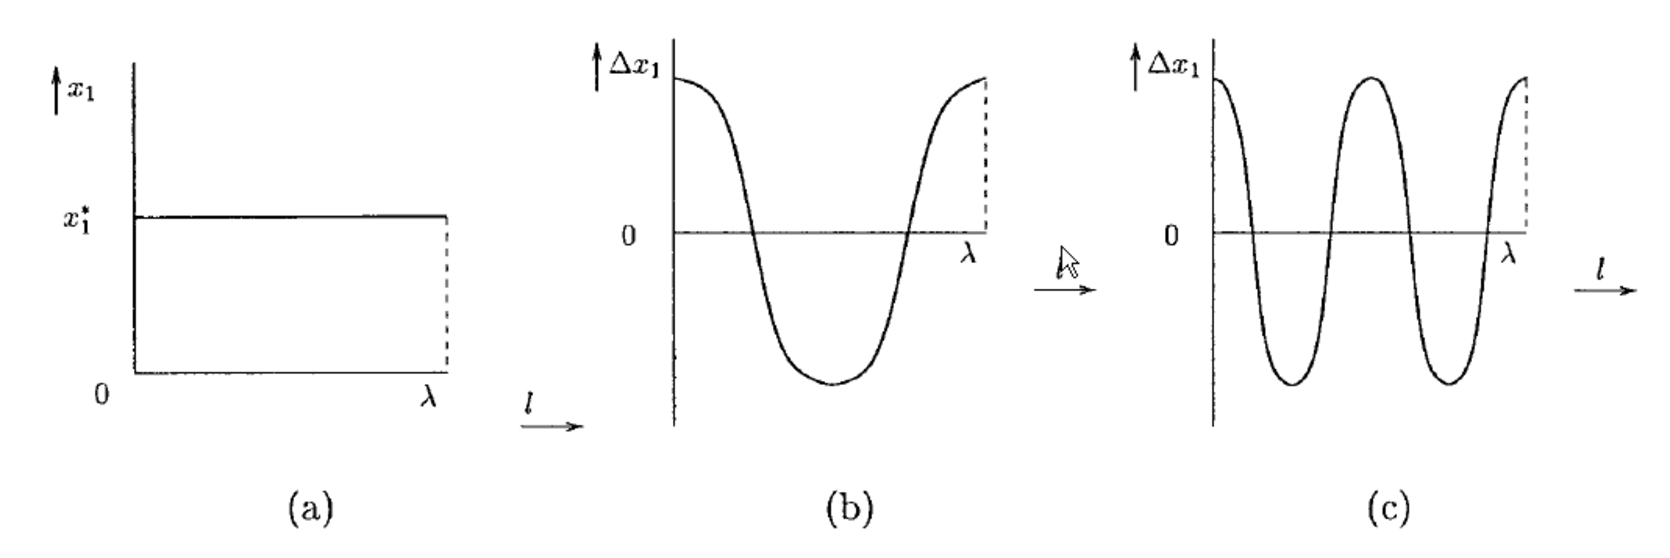
\includegraphics[width=.89\linewidth]{graphics/figure}
	\caption{This is a caption. (a) Caption caption caption, (b) Caption caption caption, (c) Caption caption caption.}
	\label{fig:figure}
\end{figure}

Add figures in the \texttt{graphics} folder.

The caption of the figure, as well as the figure, should be centered using the \texttt{\textbackslash centering\{\}} command.

To add a caption to the figure, use the \texttt{\textbackslash caption\{\}} command. 

Ensure that cross-references to figures are correct before submitting the deliverable. 

To cross-reference a figure, first create the figure using the LaTeX figure feature, then use the \texttt{\textbackslash Cref\{\}} command to reference it.

In order to cross-reference a figure, you must first add a \texttt{label} to the figure. To add a label, use the \texttt{\textbackslash label\{\}} command (see the example table above).

Add the correct path to the figure (see figure example above  \texttt{graphics/[name\_of\_the\_figure]}.


\subsubsection{Equation}
\label{sec:equation}

\textbf{Inline Equations}

To include an inline equation within a paragraph, you can use the \verb|\( ... \)| syntax:

This is an inline equation: \( E = mc^2 \).

\textbf{Display and Referencing Equations}

For the displayed equation, you can use the 
\texttt{\textbackslash begin\{equation\} ... \textbackslash end\{equation\}} syntax.

\textbf{Example of a displayed equation:}
\begin{equation}
E = mc^2 \label{eq:energy}
\end{equation}


To cross-reference an equation, first create the equation and add a label using the \texttt{\textbackslash label{}} command. Once labeled, you can reference the equation using the \texttt{\textbackslash ref{}} command (refer to the example above).

\textbf{Example:}

As seen in Equation \ref{eq:energy}, the energy of an object is related to its mass and the speed of light.

For a more formal reference with parentheses, use \(\eqref{eq:energy}\).


\subsubsection{Footnotes}
\label{sec:footnotes}

This\footnote{The footnote is at the bottom of the same page where the footnote is cited and the font size is only 9 pt. Footnotes are useful to for including nasty-looking long Web references which would look terrible if used in the main flow of the text.} is a footnote.



\subsection{Formatting Bibliographical References}
\label{sec:formatting-bibliographical-references}


By default, references use IEEE style. To add a reference, insert the BibTeX entry into \texttt{literature/references.bib}, then cite it using the \texttt{\textbackslash cite\{\}} command.


\textbf{Example}: 

Find the BibTeX entry (e.g., from Google Scholar) and add it to \texttt{literature/references.bib}

\begin{verbatim}
@article{kaloudi2020ai,
  title={The ai-based cyber threat landscape: A survey},
  author={Kaloudi, Nektaria and Li, Jingyue},
  journal={ACM Computing Surveys (CSUR)},
  volume={53},
  number={1},
  pages={1--34},
  year={2020},
  publisher={ACM New York, NY, USA}
}
\end{verbatim}

To cite in the document use: \cite{kaloudi2020ai}.




\subsection{Associated Outputs}
\label{sec:associated-outputs}

If appropriate, please include a section with details of any datasets, code or other resources being released with this deliverable.

\textbf{Example:}
The work described in this deliverable has resulted in the following resources:

\begin{center}
    \def\arraystretch{1.25}		
    \begin{tabular}{|c|c|c|}
        \hline
        \rowcolor{hyperridegray}
        \color{white} Description & 
        \color{white} URL & 
        \color{white} Availability 
        \\\hline
    
        \rowcolor{white}\color{hyperridefont} 
        My Dataset 1 &  
        \url{http://hdl.handle.net/12345} &
        Public (Apache 2.0) \\
    
        \rowcolor{hyperridelightergray}\color{hyperridefont} 
        My Dataset 2 &  
        \url{http://hdl.handle.net/54321} &
        Private (consortium only) \\
    
        \rowcolor{white}\color{hyperridefont} 
        My Code &  
        \url{https://github.com/CoEvolution-Project-EU} &
        Public (GPL3) \\
    
        \hline
    \end{tabular}
\end{center}

%%%%%%%%%%%%%%%%%%%%%%%%%%%%%%%%%%%%%%%%%
